% Options for packages loaded elsewhere
\PassOptionsToPackage{unicode}{hyperref}
\PassOptionsToPackage{hyphens}{url}
%
\documentclass[
]{article}
\usepackage{amsmath,amssymb}
\usepackage{iftex}
\ifPDFTeX
  \usepackage[T1]{fontenc}
  \usepackage[utf8]{inputenc}
  \usepackage{textcomp} % provide euro and other symbols
\else % if luatex or xetex
  \usepackage{unicode-math} % this also loads fontspec
  \defaultfontfeatures{Scale=MatchLowercase}
  \defaultfontfeatures[\rmfamily]{Ligatures=TeX,Scale=1}
\fi
\usepackage{lmodern}
\ifPDFTeX\else
  % xetex/luatex font selection
\fi
% Use upquote if available, for straight quotes in verbatim environments
\IfFileExists{upquote.sty}{\usepackage{upquote}}{}
\IfFileExists{microtype.sty}{% use microtype if available
  \usepackage[]{microtype}
  \UseMicrotypeSet[protrusion]{basicmath} % disable protrusion for tt fonts
}{}
\makeatletter
\@ifundefined{KOMAClassName}{% if non-KOMA class
  \IfFileExists{parskip.sty}{%
    \usepackage{parskip}
  }{% else
    \setlength{\parindent}{0pt}
    \setlength{\parskip}{6pt plus 2pt minus 1pt}}
}{% if KOMA class
  \KOMAoptions{parskip=half}}
\makeatother
\usepackage{xcolor}
\usepackage[margin=1in]{geometry}
\usepackage{color}
\usepackage{fancyvrb}
\newcommand{\VerbBar}{|}
\newcommand{\VERB}{\Verb[commandchars=\\\{\}]}
\DefineVerbatimEnvironment{Highlighting}{Verbatim}{commandchars=\\\{\}}
% Add ',fontsize=\small' for more characters per line
\usepackage{framed}
\definecolor{shadecolor}{RGB}{248,248,248}
\newenvironment{Shaded}{\begin{snugshade}}{\end{snugshade}}
\newcommand{\AlertTok}[1]{\textcolor[rgb]{0.94,0.16,0.16}{#1}}
\newcommand{\AnnotationTok}[1]{\textcolor[rgb]{0.56,0.35,0.01}{\textbf{\textit{#1}}}}
\newcommand{\AttributeTok}[1]{\textcolor[rgb]{0.13,0.29,0.53}{#1}}
\newcommand{\BaseNTok}[1]{\textcolor[rgb]{0.00,0.00,0.81}{#1}}
\newcommand{\BuiltInTok}[1]{#1}
\newcommand{\CharTok}[1]{\textcolor[rgb]{0.31,0.60,0.02}{#1}}
\newcommand{\CommentTok}[1]{\textcolor[rgb]{0.56,0.35,0.01}{\textit{#1}}}
\newcommand{\CommentVarTok}[1]{\textcolor[rgb]{0.56,0.35,0.01}{\textbf{\textit{#1}}}}
\newcommand{\ConstantTok}[1]{\textcolor[rgb]{0.56,0.35,0.01}{#1}}
\newcommand{\ControlFlowTok}[1]{\textcolor[rgb]{0.13,0.29,0.53}{\textbf{#1}}}
\newcommand{\DataTypeTok}[1]{\textcolor[rgb]{0.13,0.29,0.53}{#1}}
\newcommand{\DecValTok}[1]{\textcolor[rgb]{0.00,0.00,0.81}{#1}}
\newcommand{\DocumentationTok}[1]{\textcolor[rgb]{0.56,0.35,0.01}{\textbf{\textit{#1}}}}
\newcommand{\ErrorTok}[1]{\textcolor[rgb]{0.64,0.00,0.00}{\textbf{#1}}}
\newcommand{\ExtensionTok}[1]{#1}
\newcommand{\FloatTok}[1]{\textcolor[rgb]{0.00,0.00,0.81}{#1}}
\newcommand{\FunctionTok}[1]{\textcolor[rgb]{0.13,0.29,0.53}{\textbf{#1}}}
\newcommand{\ImportTok}[1]{#1}
\newcommand{\InformationTok}[1]{\textcolor[rgb]{0.56,0.35,0.01}{\textbf{\textit{#1}}}}
\newcommand{\KeywordTok}[1]{\textcolor[rgb]{0.13,0.29,0.53}{\textbf{#1}}}
\newcommand{\NormalTok}[1]{#1}
\newcommand{\OperatorTok}[1]{\textcolor[rgb]{0.81,0.36,0.00}{\textbf{#1}}}
\newcommand{\OtherTok}[1]{\textcolor[rgb]{0.56,0.35,0.01}{#1}}
\newcommand{\PreprocessorTok}[1]{\textcolor[rgb]{0.56,0.35,0.01}{\textit{#1}}}
\newcommand{\RegionMarkerTok}[1]{#1}
\newcommand{\SpecialCharTok}[1]{\textcolor[rgb]{0.81,0.36,0.00}{\textbf{#1}}}
\newcommand{\SpecialStringTok}[1]{\textcolor[rgb]{0.31,0.60,0.02}{#1}}
\newcommand{\StringTok}[1]{\textcolor[rgb]{0.31,0.60,0.02}{#1}}
\newcommand{\VariableTok}[1]{\textcolor[rgb]{0.00,0.00,0.00}{#1}}
\newcommand{\VerbatimStringTok}[1]{\textcolor[rgb]{0.31,0.60,0.02}{#1}}
\newcommand{\WarningTok}[1]{\textcolor[rgb]{0.56,0.35,0.01}{\textbf{\textit{#1}}}}
\usepackage{longtable,booktabs,array}
\usepackage{calc} % for calculating minipage widths
% Correct order of tables after \paragraph or \subparagraph
\usepackage{etoolbox}
\makeatletter
\patchcmd\longtable{\par}{\if@noskipsec\mbox{}\fi\par}{}{}
\makeatother
% Allow footnotes in longtable head/foot
\IfFileExists{footnotehyper.sty}{\usepackage{footnotehyper}}{\usepackage{footnote}}
\makesavenoteenv{longtable}
\usepackage{graphicx}
\makeatletter
\def\maxwidth{\ifdim\Gin@nat@width>\linewidth\linewidth\else\Gin@nat@width\fi}
\def\maxheight{\ifdim\Gin@nat@height>\textheight\textheight\else\Gin@nat@height\fi}
\makeatother
% Scale images if necessary, so that they will not overflow the page
% margins by default, and it is still possible to overwrite the defaults
% using explicit options in \includegraphics[width, height, ...]{}
\setkeys{Gin}{width=\maxwidth,height=\maxheight,keepaspectratio}
% Set default figure placement to htbp
\makeatletter
\def\fps@figure{htbp}
\makeatother
\usepackage{svg}
\setlength{\emergencystretch}{3em} % prevent overfull lines
\providecommand{\tightlist}{%
  \setlength{\itemsep}{0pt}\setlength{\parskip}{0pt}}
\setcounter{secnumdepth}{-\maxdimen} % remove section numbering
\ifLuaTeX
  \usepackage{selnolig}  % disable illegal ligatures
\fi
\usepackage{bookmark}
\IfFileExists{xurl.sty}{\usepackage{xurl}}{} % add URL line breaks if available
\urlstyle{same}
\hypersetup{
  pdftitle={R markdown \_ PG},
  pdfauthor={Pankaj},
  hidelinks,
  pdfcreator={LaTeX via pandoc}}

\title{R markdown \_ PG}
\author{Pankaj}
\date{2025-02-27}

\begin{document}
\maketitle

\subsection{Notes:}\label{notes}

Above line are YAML WE CAN CHANGE OUTPUT AS PER REQUIREMENT (E.G pdf,
wprd, html)

Example: output: html\_document: toc: true \# gives headers toc\_float:
true \# give header on side which we can use to navigate md\_document:
variant: gfm word\_document: pdf\_document:

OR

md\_document:\\
variant: gfm \#\#\# for github\_\_the GitHub flavored markdown (gfm) .md
file for viewing on GitHub, and we can generate a Word document as well.

\section{R code chunk}\label{r-code-chunk}

\begin{Shaded}
\begin{Highlighting}[]
\CommentTok{\#\{r R  code example1, include=FALSE\}   wont show code and output}
\CommentTok{\#\{r R  code example1, echo=FALSE\}      wont show code but output will be showm}

\CommentTok{\# this is R code}
\FunctionTok{summary}\NormalTok{(mtcars)}
\end{Highlighting}
\end{Shaded}

\begin{verbatim}
##       mpg             cyl             disp             hp       
##  Min.   :10.40   Min.   :4.000   Min.   : 71.1   Min.   : 52.0  
##  1st Qu.:15.43   1st Qu.:4.000   1st Qu.:120.8   1st Qu.: 96.5  
##  Median :19.20   Median :6.000   Median :196.3   Median :123.0  
##  Mean   :20.09   Mean   :6.188   Mean   :230.7   Mean   :146.7  
##  3rd Qu.:22.80   3rd Qu.:8.000   3rd Qu.:326.0   3rd Qu.:180.0  
##  Max.   :33.90   Max.   :8.000   Max.   :472.0   Max.   :335.0  
##       drat             wt             qsec             vs        
##  Min.   :2.760   Min.   :1.513   Min.   :14.50   Min.   :0.0000  
##  1st Qu.:3.080   1st Qu.:2.581   1st Qu.:16.89   1st Qu.:0.0000  
##  Median :3.695   Median :3.325   Median :17.71   Median :0.0000  
##  Mean   :3.597   Mean   :3.217   Mean   :17.85   Mean   :0.4375  
##  3rd Qu.:3.920   3rd Qu.:3.610   3rd Qu.:18.90   3rd Qu.:1.0000  
##  Max.   :4.930   Max.   :5.424   Max.   :22.90   Max.   :1.0000  
##        am              gear            carb      
##  Min.   :0.0000   Min.   :3.000   Min.   :1.000  
##  1st Qu.:0.0000   1st Qu.:3.000   1st Qu.:2.000  
##  Median :0.0000   Median :4.000   Median :2.000  
##  Mean   :0.4062   Mean   :3.688   Mean   :2.812  
##  3rd Qu.:1.0000   3rd Qu.:4.000   3rd Qu.:4.000  
##  Max.   :1.0000   Max.   :5.000   Max.   :8.000
\end{verbatim}

This is how to include the figures

\begin{Shaded}
\begin{Highlighting}[]
\FunctionTok{library}\NormalTok{(ggplot2)}

\FunctionTok{data}\NormalTok{(}\StringTok{"mtcars"}\NormalTok{)}
\FunctionTok{ggplot}\NormalTok{(mtcars, }\FunctionTok{aes}\NormalTok{(}\AttributeTok{x =}\NormalTok{ wt, }\AttributeTok{y =}\NormalTok{ mpg)) }\SpecialCharTok{+}
  \FunctionTok{geom\_point}\NormalTok{()}
\end{Highlighting}
\end{Shaded}

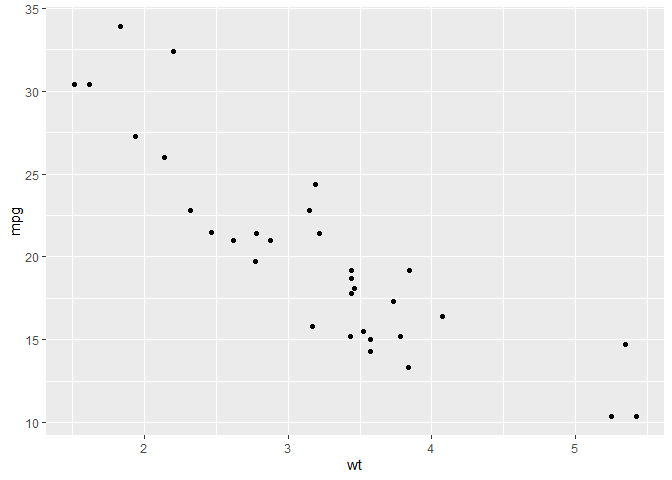
\includegraphics{Coding_practice_Rmarkdown_files/figure-latex/include the figures-1.pdf}

R markdown formatting options

\section{First level header}\label{first-level-header}

Example test

*italics test

\textbf{bold text\_between double astreix}

\begin{itemize}
\tightlist
\item
  one item
\item
  another stuff
\end{itemize}

\begin{enumerate}
\def\labelenumi{\arabic{enumi}.}
\tightlist
\item
  one item
\item
  another item
\end{enumerate}

\subsection{Second level header}\label{second-level-header}

\subsubsection{Third level header}\label{third-level-header}

\subsection{Adding the clickable
links}\label{adding-the-clickable-links}

\href{https://github.com/ppg0001/PLPA_Assignment}{Link to my GitHub}

\subsection{Images (Note can be relative pah or same
directory)}\label{images-note-can-be-relative-pah-or-same-directory}

\begin{figure}
\centering

\includegraphics{C:/Users/panka/OneDrive - Auburn University/PLPA_class/shrek.jpg}
\caption{Shrek}
\end{figure}

\subsection{Formatted tables}\label{formatted-tables}

\begin{Shaded}
\begin{Highlighting}[]
\FunctionTok{library}\NormalTok{(}\StringTok{"knitr"}\NormalTok{)}
\FunctionTok{kable}\NormalTok{(mtcars, }\AttributeTok{digits =} \DecValTok{3}\NormalTok{, }\AttributeTok{format =} \StringTok{"markdown"}\NormalTok{)}
\end{Highlighting}
\end{Shaded}

\begin{longtable}[]{@{}
  >{\raggedright\arraybackslash}p{(\columnwidth - 22\tabcolsep) * \real{0.2778}}
  >{\raggedleft\arraybackslash}p{(\columnwidth - 22\tabcolsep) * \real{0.0694}}
  >{\raggedleft\arraybackslash}p{(\columnwidth - 22\tabcolsep) * \real{0.0556}}
  >{\raggedleft\arraybackslash}p{(\columnwidth - 22\tabcolsep) * \real{0.0833}}
  >{\raggedleft\arraybackslash}p{(\columnwidth - 22\tabcolsep) * \real{0.0556}}
  >{\raggedleft\arraybackslash}p{(\columnwidth - 22\tabcolsep) * \real{0.0694}}
  >{\raggedleft\arraybackslash}p{(\columnwidth - 22\tabcolsep) * \real{0.0833}}
  >{\raggedleft\arraybackslash}p{(\columnwidth - 22\tabcolsep) * \real{0.0833}}
  >{\raggedleft\arraybackslash}p{(\columnwidth - 22\tabcolsep) * \real{0.0417}}
  >{\raggedleft\arraybackslash}p{(\columnwidth - 22\tabcolsep) * \real{0.0417}}
  >{\raggedleft\arraybackslash}p{(\columnwidth - 22\tabcolsep) * \real{0.0694}}
  >{\raggedleft\arraybackslash}p{(\columnwidth - 22\tabcolsep) * \real{0.0694}}@{}}
\toprule\noalign{}
\begin{minipage}[b]{\linewidth}\raggedright
\end{minipage} & \begin{minipage}[b]{\linewidth}\raggedleft
mpg
\end{minipage} & \begin{minipage}[b]{\linewidth}\raggedleft
cyl
\end{minipage} & \begin{minipage}[b]{\linewidth}\raggedleft
disp
\end{minipage} & \begin{minipage}[b]{\linewidth}\raggedleft
hp
\end{minipage} & \begin{minipage}[b]{\linewidth}\raggedleft
drat
\end{minipage} & \begin{minipage}[b]{\linewidth}\raggedleft
wt
\end{minipage} & \begin{minipage}[b]{\linewidth}\raggedleft
qsec
\end{minipage} & \begin{minipage}[b]{\linewidth}\raggedleft
vs
\end{minipage} & \begin{minipage}[b]{\linewidth}\raggedleft
am
\end{minipage} & \begin{minipage}[b]{\linewidth}\raggedleft
gear
\end{minipage} & \begin{minipage}[b]{\linewidth}\raggedleft
carb
\end{minipage} \\
\midrule\noalign{}
\endhead
\bottomrule\noalign{}
\endlastfoot
Mazda RX4 & 21.0 & 6 & 160.0 & 110 & 3.90 & 2.620 & 16.46 & 0 & 1 & 4 &
4 \\
Mazda RX4 Wag & 21.0 & 6 & 160.0 & 110 & 3.90 & 2.875 & 17.02 & 0 & 1 &
4 & 4 \\
Datsun 710 & 22.8 & 4 & 108.0 & 93 & 3.85 & 2.320 & 18.61 & 1 & 1 & 4 &
1 \\
Hornet 4 Drive & 21.4 & 6 & 258.0 & 110 & 3.08 & 3.215 & 19.44 & 1 & 0 &
3 & 1 \\
Hornet Sportabout & 18.7 & 8 & 360.0 & 175 & 3.15 & 3.440 & 17.02 & 0 &
0 & 3 & 2 \\
Valiant & 18.1 & 6 & 225.0 & 105 & 2.76 & 3.460 & 20.22 & 1 & 0 & 3 &
1 \\
Duster 360 & 14.3 & 8 & 360.0 & 245 & 3.21 & 3.570 & 15.84 & 0 & 0 & 3 &
4 \\
Merc 240D & 24.4 & 4 & 146.7 & 62 & 3.69 & 3.190 & 20.00 & 1 & 0 & 4 &
2 \\
Merc 230 & 22.8 & 4 & 140.8 & 95 & 3.92 & 3.150 & 22.90 & 1 & 0 & 4 &
2 \\
Merc 280 & 19.2 & 6 & 167.6 & 123 & 3.92 & 3.440 & 18.30 & 1 & 0 & 4 &
4 \\
Merc 280C & 17.8 & 6 & 167.6 & 123 & 3.92 & 3.440 & 18.90 & 1 & 0 & 4 &
4 \\
Merc 450SE & 16.4 & 8 & 275.8 & 180 & 3.07 & 4.070 & 17.40 & 0 & 0 & 3 &
3 \\
Merc 450SL & 17.3 & 8 & 275.8 & 180 & 3.07 & 3.730 & 17.60 & 0 & 0 & 3 &
3 \\
Merc 450SLC & 15.2 & 8 & 275.8 & 180 & 3.07 & 3.780 & 18.00 & 0 & 0 & 3
& 3 \\
Cadillac Fleetwood & 10.4 & 8 & 472.0 & 205 & 2.93 & 5.250 & 17.98 & 0 &
0 & 3 & 4 \\
Lincoln Continental & 10.4 & 8 & 460.0 & 215 & 3.00 & 5.424 & 17.82 & 0
& 0 & 3 & 4 \\
Chrysler Imperial & 14.7 & 8 & 440.0 & 230 & 3.23 & 5.345 & 17.42 & 0 &
0 & 3 & 4 \\
Fiat 128 & 32.4 & 4 & 78.7 & 66 & 4.08 & 2.200 & 19.47 & 1 & 1 & 4 &
1 \\
Honda Civic & 30.4 & 4 & 75.7 & 52 & 4.93 & 1.615 & 18.52 & 1 & 1 & 4 &
2 \\
Toyota Corolla & 33.9 & 4 & 71.1 & 65 & 4.22 & 1.835 & 19.90 & 1 & 1 & 4
& 1 \\
Toyota Corona & 21.5 & 4 & 120.1 & 97 & 3.70 & 2.465 & 20.01 & 1 & 0 & 3
& 1 \\
Dodge Challenger & 15.5 & 8 & 318.0 & 150 & 2.76 & 3.520 & 16.87 & 0 & 0
& 3 & 2 \\
AMC Javelin & 15.2 & 8 & 304.0 & 150 & 3.15 & 3.435 & 17.30 & 0 & 0 & 3
& 2 \\
Camaro Z28 & 13.3 & 8 & 350.0 & 245 & 3.73 & 3.840 & 15.41 & 0 & 0 & 3 &
4 \\
Pontiac Firebird & 19.2 & 8 & 400.0 & 175 & 3.08 & 3.845 & 17.05 & 0 & 0
& 3 & 2 \\
Fiat X1-9 & 27.3 & 4 & 79.0 & 66 & 4.08 & 1.935 & 18.90 & 1 & 1 & 4 &
1 \\
Porsche 914-2 & 26.0 & 4 & 120.3 & 91 & 4.43 & 2.140 & 16.70 & 0 & 1 & 5
& 2 \\
Lotus Europa & 30.4 & 4 & 95.1 & 113 & 3.77 & 1.513 & 16.90 & 1 & 1 & 5
& 2 \\
Ford Pantera L & 15.8 & 8 & 351.0 & 264 & 4.22 & 3.170 & 14.50 & 0 & 1 &
5 & 4 \\
Ferrari Dino & 19.7 & 6 & 145.0 & 175 & 3.62 & 2.770 & 15.50 & 0 & 1 & 5
& 6 \\
Maserati Bora & 15.0 & 8 & 301.0 & 335 & 3.54 & 3.570 & 14.60 & 0 & 1 &
5 & 8 \\
Volvo 142E & 21.4 & 4 & 121.0 & 109 & 4.11 & 2.780 & 18.60 & 1 & 1 & 4 &
2 \\
\end{longtable}

\subsection{\texorpdfstring{\textbf{Organizing a repository and editing
a readme using
Markdown}}{Organizing a repository and editing a readme using Markdown}}\label{organizing-a-repository-and-editing-a-readme-using-markdown}

\section{PLPA\_Repository}\label{plpa_repository}

This is repository for PLPA class. I use it store my assignments and to
try different tutorials.

\section{DOI}\label{doi}

\href{https://doi.org/10.5281/zenodo.14935003}{\includesvg{https://zenodo.org/badge/924493573.svg}}

\subsection{\texorpdfstring{\textbf{Organizing a repository and editing
a readme using
Markdown}}{Organizing a repository and editing a readme using Markdown}}\label{organizing-a-repository-and-editing-a-readme-using-markdown-1}

\paragraph{Instead of dummy I will arrange this
repository}\label{instead-of-dummy-i-will-arrange-this-repository}

\begin{itemize}
\tightlist
\item
  \href{https://github.com/ppg0001/PLPA_Assignment}{Click here to visit
  the Repository} Note: This is my regular repository I use for class
  assignments.
\end{itemize}

\subsubsection{\texorpdfstring{\textbf{Link to
analysis}}{Link to analysis}}\label{link-to-analysis}

\begin{itemize}
\tightlist
\item
  \href{Coding_practice_Rmarkdown.md}{Analysis 1}
\end{itemize}

Note: can add more links to the analysis by adding respective relative
paths. So it is organized with clickable links to analysis.

\subsubsection{\texorpdfstring{\textbf{File
Tree}}{File Tree}}\label{file-tree}

Use package fs for file tree (In terminal: install.packages(``fs'')

\textbf{Code:} fs::dir\_tree()\\
Note: This will print the directory structure since I am in my root
directory. OR can specify the directory path in brackets.

\begin{Shaded}
\begin{Highlighting}[]
\FunctionTok{install.packages}\NormalTok{(}\StringTok{"fs"}\NormalTok{)}
\NormalTok{fs}\SpecialCharTok{::}\FunctionTok{dir\_tree}\NormalTok{()}
\end{Highlighting}
\end{Shaded}

To add text in box use: forward single quotes \textbf{```} Note good
habit to describe folders/file in the below structure (example\#)

\begin{verbatim}
── Coding Pracitce Assignment2_Datavis1    #Assignment2 folder
│   ├── Assignment_DataVis1.docx
│   ├── Assingmner_DataVis2.pdf
│   ├── Bull_richness.csv                 # Raw data for analysis for assignment2
│   └── Coding_Assignment2_DataVis.R
├── Coding Practice Assignment1_Intro     #Assignment folder
│   ├── PLPA_assignment_R1.R
│   └── TipsR.csv
├── CodingChalleng3_AdvancedVis.R
├── CodingChallenge2_IntroDataVis.R
├── Coding_Challenge1_Assignment_.R
├── Coding_practice_Rmarkdown.html
├── Coding_practice_Rmarkdown.md
├── Coding_practice_Rmarkdown.Rmd
├── Coding_practice_Rmarkdown_files
│   └── figure-gfm
│       └── include the figures-1.png
├── Dummy_markdown_repo_edit_PG.Rmd
├── MycotoxinData.csv
├── PLPA_Assignment.Rproj                  # Top level directory .Rproj file = Working directory
├── README.html
├── README.md                             #Top level directory README
└── shrek.jpg
\end{verbatim}

\subsubsection{\texorpdfstring{\textbf{Zendo}}{Zendo}}\label{zendo}

DOI created by zenodo:
\href{https://doi.org/10.5281/zenodo.14935003}{\includesvg{https://zenodo.org/badge/924493573.svg}}

\end{document}
